\documentclass{standalone}

\usepackage[T1]{fontenc}
\usepackage[utf8]{inputenc}

\usepackage{pgf-umlcd}

\begin{document}

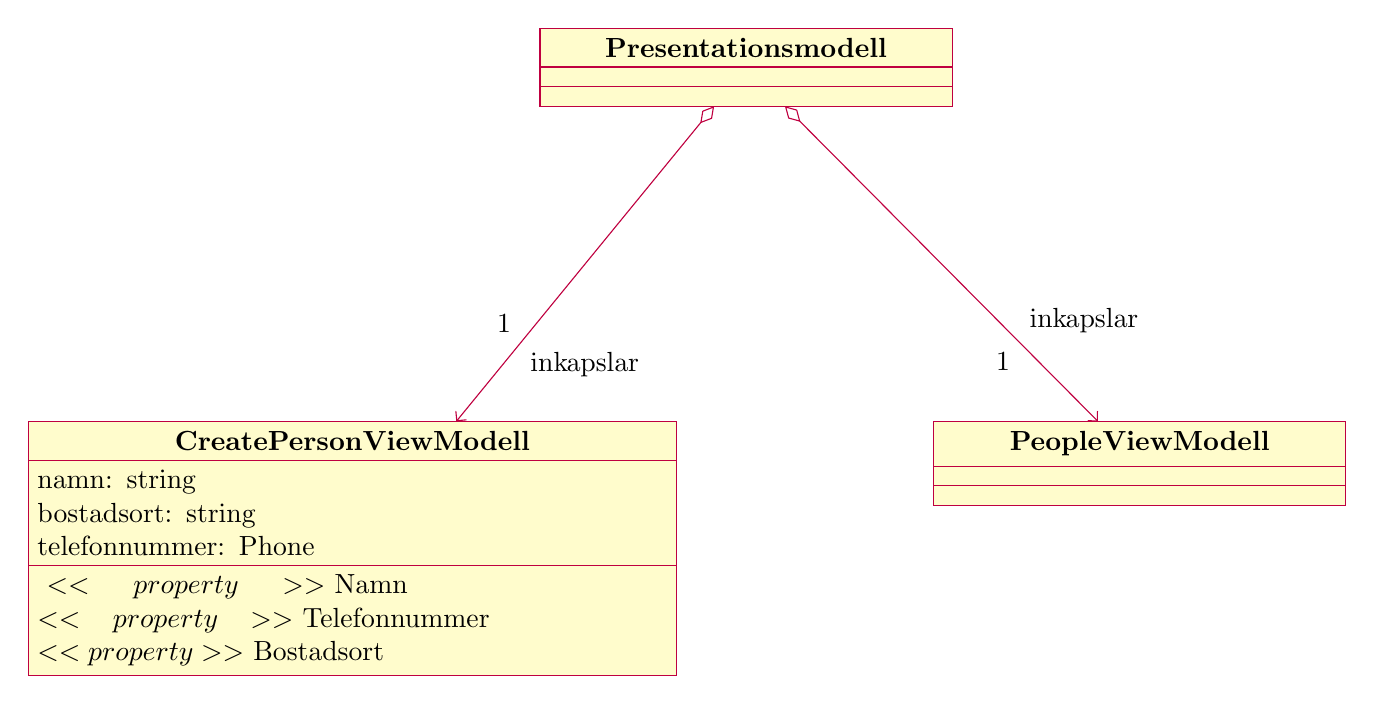
\begin{tikzpicture}
  \begin{class}[text width=5cm]{PeopleViewModell}{5,-5}

  \end{class}

  \begin{class}[text width=8cm]{CreatePersonViewModell}{-5,-5}
    \attribute{namn: string}
    \attribute{bostadsort: string}
    \attribute{telefonnummer: Phone}

    \operation{ $<<property>>$ Namn}
    \operation{ $<<property>>$ Telefonnummer}
    \operation{ $<<property>>$ Bostadsort}
  \end{class}

  \begin{class}[text width=5cm]{Presentationsmodell}{0,0}

  \end{class}

  \aggregation{Presentationsmodell}{inkapslar}{1}{PeopleViewModell};
  \aggregation{Presentationsmodell}{inkapslar}{1}{CreatePersonViewModell};
  %% \umlnote (note) (-3, -3) {eftersom en view hanterar en modell};
\end{tikzpicture}

\end{document}
